%============================================================
%  ENTREGA I — SECCIONES 1 a 6 (cuerpo)
%  Requiere el preámbulo del plan: tabularx (col. L{} e Y),
%  booktabs, xcolor, hyperref, tikz, graphicx, enumitem.
%============================================================

%------------------------------------------------------------------
\FloatBarrier
\section*{1. Información general del proyecto}
\phantomsection\addcontentsline{toc}{section}{1. Información general del proyecto}

El sistema bajo prueba es \textbf{Demoblaze}, un sitio de terceros publicado por
BlazeMeter. El equipo no tiene su código fuente ni acceso al servidor, a la base de
datos o a los registros de aplicación: solo lo prueba por caja negra desde el
navegador. Por eso, las secciones que describen cómo está construido el sistema —en
especial la arquitectura— se basan en lo que se observa desde afuera (el tráfico HTTP
y los recursos que carga el navegador) y no en documentación interna del proveedor.

\begingroup
\small
\renewcommand{\arraystretch}{1.25}
\begin{table}[htb]\centering\small
\caption{Datos generales del proyecto y del sistema bajo prueba.}\label{tab:info-general}
\begin{tabularx}{\textwidth}{@{}L{4.4cm} Y@{}}
\toprule
\textbf{Elemento} & \textbf{Detalle} \\
\midrule
Nombre del software & Demoblaze \\
Tipo de sistema & Comercio electrónico: tienda en línea de demostración (\emph{demo e-commerce}). \\
URL de la aplicación & \url{https://www.demoblaze.com} \\
API que consume & \url{https://api.demoblaze.com} \\
Proveedor & BlazeMeter \\
Curso & Construcción de Software y Pruebas — Grupo A — 2026-2 \\
Profesora & Claudia Martínez \\
Institución & Pontificia Universidad Javeriana Cali \\
Entrega & Entrega I (100 pts) — fecha de entrega: 22 de octubre de 2026 \\
\bottomrule
\end{tabularx}
\end{table}
\endgroup

\subsection*{1.1 Integrantes del equipo}
\addcontentsline{toc}{subsection}{1.1 Integrantes del equipo}

\begingroup
\small
\renewcommand{\arraystretch}{1.25}
\begin{table}[htb]\centering\small
\caption{Integrantes del equipo.}\label{tab:integrantes}
\begin{tabularx}{\textwidth}{@{}L{6cm} Y@{}}
\toprule
\textbf{Integrante} & \textbf{Rol en la entrega} \\
\midrule
Joshua Mendez & Integrante \\
Edinson Pedroza & Integrante \\
\bottomrule
\end{tabularx}
\end{table}
\endgroup

\subsection*{1.2 Repositorio del código}
\addcontentsline{toc}{subsection}{1.2 Repositorio del código}

Aquí hay que hacer una distinción, porque el sistema bajo prueba no es del equipo.

\begin{itemize}
  \item \textbf{Código fuente de Demoblaze (el SUT): no disponible.} Demoblaze es un
        sitio de demostración de BlazeMeter, pensado para practicar automatización y
        QA. Su código fuente no es público y el equipo no tiene acceso al repositorio
        del proveedor, al servidor ni a la base de datos. Todo el trabajo se hace por
        caja negra desde el navegador. No se referencia ninguna URL de repositorio de
        Demoblaze porque no existe una pública que corresponda a este sistema.
  \item \textbf{Repositorio del equipo (artefactos de prueba): sí existe.} Lo que el
        equipo sí versiona es su propio trabajo: la suite de casos de prueba, el plan
        de pruebas, el registro de ejecución, los reportes de defectos y las
        evidencias. Ese es el repositorio que acompaña esta entrega.
\end{itemize}

\begingroup
\small
\renewcommand{\arraystretch}{1.25}
\begin{table}[htb]\centering\small
\caption{Repositorio de artefactos de prueba del equipo.}\label{tab:repo}
\begin{tabularx}{\textwidth}{@{}L{4.4cm} Y@{}}
\toprule
\textbf{Elemento} & \textbf{Valor} \\
\midrule
Repositorio del equipo (artefactos de prueba) & \url{https://github.com/JoshuaMontclair/demoblaze-pruebas-entrega1} \\
Contenido del repositorio & Suite de 68 casos de prueba (60 del plan + 8 de arreglos ortogonales), plan de pruebas, registro de ejecución, reportes de defectos y evidencias gráficas. \\
\bottomrule
\end{tabularx}
\end{table}
\endgroup

\noindent\emph{El repositorio contiene los artefactos de pruebas del equipo, no el código de Demoblaze (software de terceros).}

%------------------------------------------------------------------
\FloatBarrier
\section*{2. Descripción del sistema}
\phantomsection\addcontentsline{toc}{section}{2. Descripción del sistema}

\textbf{Qué es.} Demoblaze es una tienda en línea de demostración: reproduce el
comportamiento de un comercio electrónico real —catálogo de productos, detalle de
producto, carrito, registro, inicio de sesión y orden de compra— pero sin vender nada
de verdad ni cobrar pagos reales. Es un entorno de práctica estable y de acceso libre.

\textbf{Qué problema resuelve.} No resuelve un problema comercial; resuelve un problema
de formación y de herramientas. Quien aprende o ejercita pruebas de software necesita
un sistema realista contra el cual trabajar, que tenga flujos completos (navegar,
agregar al carrito, autenticarse, comprar) y que no imponga el riesgo de operar sobre
un sistema productivo real con datos o dinero de clientes. Demoblaze ofrece exactamente
eso: un e-commerce funcional, público y gratuito, que sirve de banco de pruebas para
diseñar casos, automatizar flujos y validar técnicas de testing.

\textbf{Quiénes lo usan.} Sus usuarios no son compradores reales, sino personas que
practican o enseñan calidad de software: estudiantes de pruebas, ingenieros de QA que
ensayan herramientas de automatización (Selenium, Playwright, Katalon y similares),
instructores que necesitan un sistema de ejemplo y equipos que evalúan frameworks de
prueba. Para el presente proyecto, el equipo lo usa como sistema bajo prueba de la
asignatura.

\textbf{Qué valor ofrece.} Un ambiente de práctica fiel a un comercio electrónico real,
disponible sin costo y sin necesidad de montar infraestructura propia. Al imitar los
módulos y las reglas de negocio de una tienda —el total es la suma de los ítems del
carrito, no se compra con el carrito vacío, el precio del listado coincide con el del
detalle— permite ejercitar pruebas funcionales, de integración de interfaz con
servicio, de seguridad básica y de rendimiento sobre un objetivo representativo. Que
sea un sistema de terceros, en producción y sin posibilidad de corregir sus defectos,
es parte de lo que lo hace un buen ejercicio: obliga a probar y documentar la calidad
observable desde afuera, que es la situación habitual cuando se audita un producto que
uno no construyó.

%------------------------------------------------------------------
\FloatBarrier
\section*{3. Arquitectura general}
\phantomsection\addcontentsline{toc}{section}{3. Arquitectura general}

La arquitectura que se describe aquí es la \textbf{inferida a partir de lo observable
desde el exterior}: el tráfico HTTP del navegador, los recursos que la página carga y
las respuestas del servicio. Al no tener acceso al código ni a la infraestructura del
proveedor, no se documenta la implementación interna (lenguaje del servidor, motor de
base de datos, despliegue), sino la forma en que el cliente y el servicio se comunican
tal como se ve desde el navegador.

\subsection*{3.1 Tecnologías observadas}
\addcontentsline{toc}{subsection}{3.1 Tecnologías observadas}

\begin{itemize}
  \item \textbf{Cliente web (frontend).} Es una aplicación de página única (SPA)
        servida como contenido estático desde \texttt{www.demoblaze.com}. Está
        construida con HTML, CSS y JavaScript, apoyada en \textbf{jQuery} para la
        manipulación del DOM y las llamadas al servicio, y en \textbf{Bootstrap} para
        la maquetación y los componentes visuales (grilla, modales, carrusel). La
        interfaz no calcula la lógica de negocio por su cuenta: delega en el servicio
        HTTP y pinta lo que este responde.
  \item \textbf{Servicio (backend).} Una \textbf{API HTTP de estilo REST} en
        \texttt{api.demoblaze.com} que responde en \textbf{JSON}. El frontend la
        consume para listar productos, filtrar por categoría, cargar el detalle de un
        producto, autenticar y operar el carrito y la orden. Entre las llamadas
        observadas en el tráfico están \texttt{GET /entries} (listado de productos),
        \texttt{POST /bycat} (productos por categoría), \texttt{POST /view} (detalle
        por identificador) y el servicio de \texttt{login}. Las operaciones de carrito
        y de compra también pasan por esta API.
  \item \textbf{Autenticación por token.} El inicio de sesión se resuelve contra el
        servicio: ante credenciales válidas, la API devuelve un \textbf{token de
        sesión} que el cliente usa para las operaciones que requieren usuario
        autenticado. (En el tráfico del login se observó, además, que la contraseña
        viaja codificada en base64 sobre HTTPS; esto es un hallazgo de seguridad
        documentado en el plan de pruebas, no una característica de diseño
        recomendable.)
  \item \textbf{Almacén de datos.} No es accesible ni inspeccionable, pero su
        existencia se infiere de que la API mantiene y devuelve de forma consistente
        los productos, categorías, usuarios registrados, el contenido del carrito y
        las órdenes. Se representa como un componente lógico ``almacén de datos''
        detrás de la API.
\end{itemize}

\subsection*{3.2 Componentes principales}
\addcontentsline{toc}{subsection}{3.2 Componentes principales}

\begin{enumerate}
  \item \textbf{Cliente web (SPA).} El navegador del usuario carga la página y sus
        recursos estáticos (HTML, JS, CSS, imágenes y el video de \emph{About us}) y
        ejecuta la lógica de presentación.
  \item \textbf{API REST.} Recibe las peticiones HTTP del cliente, devuelve JSON y
        concentra la lógica de negocio (catálogo, carrito, autenticación, compra).
  \item \textbf{Almacén de datos.} Guarda y provee la información que la API expone.
\end{enumerate}

La separación es nítida: el cliente es ``tonto'' respecto del negocio y el servicio es
quien decide. Esto quedó en evidencia durante las pruebas de integración, donde la
interfaz mostró \emph{undefined} al confiar en una respuesta \texttt{200 OK} que en
realidad traía \texttt{\{"errorMessage":"Not found."\}} para un producto inexistente
—es decir, el cliente pinta lo que el servicio le entrega sin validarlo por su cuenta.

\subsection*{3.3 Diagrama de arquitectura}
\addcontentsline{toc}{subsection}{3.3 Diagrama de arquitectura}

El flujo va de izquierda a derecha (Figura~\ref{fig:arquitectura}). Los componentes con
borde continuo (SPA, servidor estático y API) se \textbf{observan directamente} en el
tráfico del navegador; el almacén de datos va con borde punteado porque es un
componente \textbf{inferido}: no se inspecciona, pero su existencia se deduce de la
consistencia de las respuestas. El recuadro ``Infraestructura de BlazeMeter — caja
negra'' agrupa todo lo que es del proveedor y a lo que el equipo no tiene acceso.

\usetikzlibrary{arrows.meta,positioning,fit,backgrounds}
\begin{figure}[htb]\centering
\resizebox{\textwidth}{!}{%
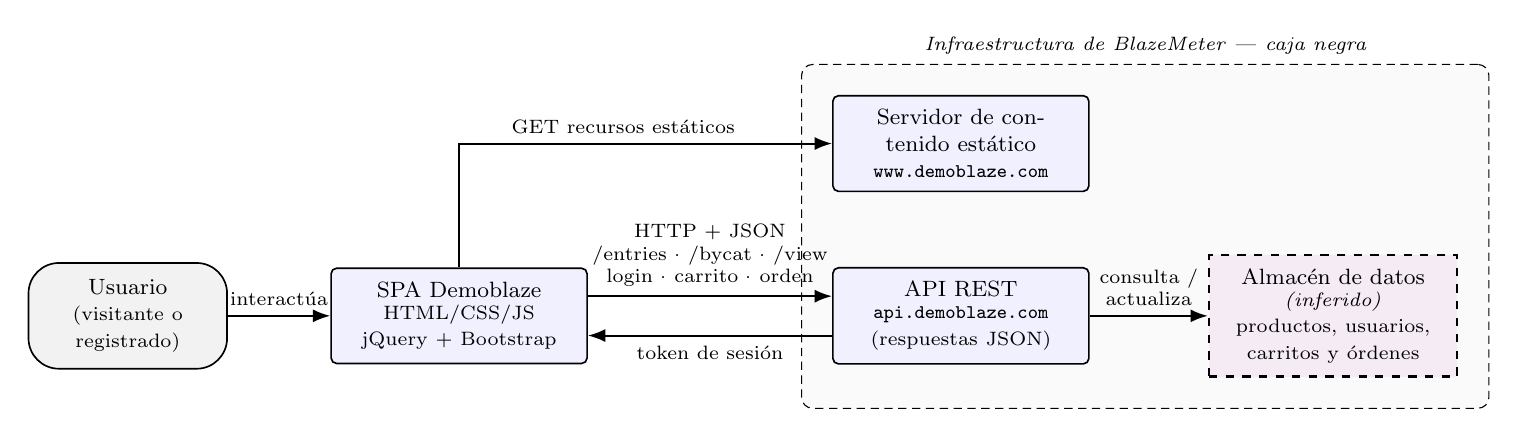
\begin{tikzpicture}[
  font=\footnotesize,
  >={Latex[length=2.2mm]},
  box/.style   ={draw,rounded corners=2pt,align=center,inner sep=5pt,
                 fill=blue!6,line width=0.6pt,text width=2.9cm},
  store/.style ={draw,dashed,align=center,inner sep=5pt,
                 fill=violet!8,line width=0.9pt,text width=2.8cm},
  actor/.style ={draw,rounded corners=11pt,align=center,inner sep=6pt,
                 fill=gray!10,line width=0.6pt,text width=2.1cm},
  flow/.style  ={->,line width=0.7pt},
]
  \node[actor] (user) {Usuario\\\scriptsize(visitante o registrado)};
  \node[box, right=1.3cm of user]  (spa)      {SPA Demoblaze\\\scriptsize HTML/CSS/JS\\\scriptsize jQuery + Bootstrap};
  \node[box, right=3.1cm of spa]   (api)      {API REST\\\scriptsize\texttt{api.demoblaze.com}\\\scriptsize (respuestas JSON)};
  \node[box, above=0.95cm of api]  (estatico) {Servidor de contenido estático\\\scriptsize\texttt{www.demoblaze.com}};
  \node[store, right=1.5cm of api] (datos)    {Almacén de datos\\\scriptsize\textit{(inferido)}\\\scriptsize productos, usuarios, carritos y órdenes};

  \draw[flow] (user) -- node[above,font=\scriptsize]{interactúa} (spa);
  \draw[flow] (spa.north) |- node[above,pos=0.72,font=\scriptsize]{GET recursos estáticos} (estatico.west);
  \draw[flow] ([yshift=2.5mm]spa.east) -- node[above,align=center,font=\scriptsize]{HTTP + JSON\\/entries · /bycat · /view\\login · carrito · orden} ([yshift=2.5mm]api.west);
  \draw[flow] ([yshift=-2.5mm]api.west) -- node[below,font=\scriptsize]{token de sesión} ([yshift=-2.5mm]spa.east);
  \draw[flow] (api) -- node[above,align=center,font=\scriptsize]{consulta /\\actualiza} (datos);

  \begin{scope}[on background layer]
    \node[draw,dash pattern=on 3pt off 2pt,rounded corners,fill=gray!4,
          inner sep=11pt,fit=(estatico)(api)(datos),
          label={[font=\scriptsize\itshape]above:Infraestructura de BlazeMeter — caja negra}] {};
  \end{scope}
\end{tikzpicture}%
}
\caption{Arquitectura observada/inferida de Demoblaze. El cliente delega toda la lógica
de negocio en la API REST; el almacén de datos (borde punteado) es un componente
inferido a partir de la consistencia de las respuestas.}\label{fig:arquitectura}
\end{figure}

\subsection*{3.4 Descripción del diagrama (en prosa)}
\addcontentsline{toc}{subsection}{3.4 Descripción del diagrama (en prosa)}

El flujo va de izquierda a derecha. El \textbf{usuario} —sea visitante sin sesión o
usuario registrado— interactúa con la \textbf{SPA de Demoblaze} que se ejecuta en su
propio navegador. Esa aplicación de página única es HTML, CSS y JavaScript con jQuery y
Bootstrap, y se descarga como contenido estático desde \texttt{www.demoblaze.com}
(flecha de recursos estáticos hacia el \emph{servidor de contenido estático}).

Toda la lógica de negocio ocurre en el segundo salto: la SPA hace peticiones
\textbf{HTTP} a la \textbf{API REST} de \texttt{api.demoblaze.com}, que responde en
\textbf{JSON}. Por ese canal pasan el listado de productos (\texttt{/entries}), el
filtrado por categoría (\texttt{/bycat}), el detalle de producto (\texttt{/view}), el
inicio de sesión y las operaciones de carrito y de orden de compra. Cuando el usuario
se autentica correctamente, la API le devuelve a la SPA un \textbf{token de sesión},
que habilita las acciones propias del usuario registrado. Finalmente, la API consulta y
actualiza un \textbf{almacén de datos} que guarda productos, usuarios, carritos y
órdenes.

En el diagrama, los componentes con borde continuo (SPA, servidor estático y API) son
los que se \textbf{observan directamente} en el tráfico del navegador; el almacén de
datos va con borde punteado porque es un componente \textbf{inferido}: no se
inspecciona, pero su existencia se deduce de la consistencia de las respuestas. El
recuadro ``Infraestructura de BlazeMeter — caja negra'' agrupa todo lo que es del
proveedor y a lo que el equipo no tiene acceso.

%------------------------------------------------------------------
\FloatBarrier
\section*{4. Actores / tipos de usuario}
\phantomsection\addcontentsline{toc}{section}{4. Actores / tipos de usuario}

Demoblaze distingue, desde afuera, dos tipos de usuario según tengan o no una sesión
iniciada. No existe un panel de administrador accesible públicamente, así que no se
considera un tercer actor administrador.

\subsection*{4.1 Usuario visitante (sin sesión)}
\addcontentsline{toc}{subsection}{4.1 Usuario visitante (sin sesión)}

Es cualquier persona que entra al sitio sin autenticarse. Puede recorrer y operar casi
toda la tienda:

\begin{itemize}
  \item Ver el \textbf{catálogo} de productos en la página principal.
  \item Filtrar por las tres \textbf{categorías}: Phones, Laptops y Monitors.
  \item Navegar la \textbf{paginación} del listado.
  \item Abrir el \textbf{detalle} de un producto (nombre, precio, descripción e
        imagen).
  \item \textbf{Agregar productos al carrito} y ver el carrito, con el total como suma
        de los ítems, y la persistencia del contenido al navegar entre páginas.
  \item Eliminar productos del carrito.
  \item Abrir el formulario de \textbf{orden de compra} (Place Order), que presenta el
        total precargado y seis campos editables (Name, Country, City, Credit card,
        Month, Year).
  \item Enviar el formulario de \textbf{Contacto} (email, nombre, mensaje).
  \item \textbf{Registrarse} (Sign up) para crear una cuenta.
\end{itemize}

\subsection*{4.2 Usuario registrado (con sesión)}
\addcontentsline{toc}{subsection}{4.2 Usuario registrado (con sesión)}

Es el visitante que creó una cuenta (Sign up) y además inició sesión (Log in). La
sesión se sostiene mediante el token que devuelve la API. Además de todo lo que puede
hacer el visitante, el usuario registrado:

\begin{itemize}
  \item Opera el sitio con su \textbf{sesión identificada} (su nombre de usuario queda
        visible en la barra superior).
  \item Puede \textbf{cerrar sesión} (Log out).
  \item Completa el flujo de compra asociado a su cuenta.
\end{itemize}

\noindent\emph{Sobre la sesión y la compra (comportamiento real observado).} El sitio
permite abrir el formulario \emph{Place Order} y procede a validar sus campos antes que
la sesión: con el carrito vacío no deja completar la compra (regla R1), y en el
formulario, si faltan Name o Credit card, el sistema la rechaza con el mensaje
\texttt{Please fill out Name and Creditcard.} (regla R5). El comportamiento exacto
respecto de la sesión en el momento de confirmar la compra se documenta en el plan de
pruebas con su evidencia; aquí se describe el flujo tal como se observa desde la
interfaz.

\subsection*{4.3 Administrador}
\addcontentsline{toc}{subsection}{4.3 Administrador}

\textbf{No hay un actor administrador accesible públicamente.} Demoblaze no expone una
consola de administración ni funciones de gestión (altas de productos, gestión de
usuarios, reportes) a las que el equipo pueda llegar desde el navegador. Cualquier
administración del sitio es interna al proveedor (BlazeMeter) y queda fuera del alcance
observable, por lo que no se modela como actor del sistema bajo prueba.

%------------------------------------------------------------------
\FloatBarrier
\section*{5. Lista de funcionalidades del sistema}
\phantomsection\addcontentsline{toc}{section}{5. Lista de funcionalidades del sistema}

Una funcionalidad \textbf{con lógica de negocio} es aquella en la que el sistema aplica
un cálculo, una validación compuesta, un algoritmo de selección o una regla de
consistencia; no se limita a crear, leer, actualizar o borrar un registro. A
continuación se identifican cuatro funcionalidades de Demoblaze que cumplen ese
criterio.

\begingroup
\footnotesize
\setlength{\tabcolsep}{4pt}
\renewcommand{\arraystretch}{1.2}
\begin{table}[htb]\centering\footnotesize
\caption{Funcionalidades con lógica de negocio (no-CRUD).}\label{tab:funcionalidades}
\begin{tabularx}{\textwidth}{@{}c L{2.4cm} L{2.2cm} Y@{}}
\toprule
\textbf{\#} & \textbf{Funcionalidad} & \textbf{Actor} & \textbf{Descripción (lógica que la hace no-CRUD)} \\
\midrule
F1 & \textbf{Cálculo del total del carrito} & Cliente (comprador) &
El sistema no almacena un total fijo: lo \textbf{calcula} sumando el precio de cada
ítem presente en el carrito cada vez que se agrega o elimina un producto. El resultado
es una operación aritmética derivada del contenido actual del carrito, no un dato que
el usuario introduzca o edite. La prueba verifica que el total es igual a la suma de
los precios de los ítems ($\mathrm{TOTAL} = \sum$ precios) para uno y varios
productos (regla R3). \\
F2 & \textbf{Validación del flujo de compra (Place Order)} & Cliente (comprador, en sesión) &
El sitio decide si una compra procede combinando \textbf{tres condiciones}: que haya
una sesión iniciada, que el carrito no esté vacío y que los campos obligatorios estén
completos. Solo con las tres satisfechas se genera el comprobante; si falta cualquiera,
rechaza. Es una \textbf{validación compuesta} (modelada como tabla de decisión), no la
simple escritura de un formulario. Incorpora además la \textbf{precarga del total}
desde el carrito y las obligatoriedades de R1, R2 y R5. \\
F3 & \textbf{Filtrado del catálogo por categoría} & Visitante / Cliente &
Sobre el listado de productos, el sistema \textbf{selecciona y reconstruye} el conjunto
mostrado según la categoría elegida (Phones, Laptops, Monitors), pidiendo al servicio
solo los productos de esa clase y repintando la página. Es un \textbf{algoritmo de
filtrado} con un criterio de pertenencia, no la lectura plana de una lista completa. \\
F4 & \textbf{Consistencia de precio entre listado y detalle} & Visitante / Cliente &
El sistema expone el precio de un mismo producto en dos vistas (tarjeta del catálogo y
ficha de detalle) que se nutren del mismo servicio. La funcionalidad relevante es que
esos dos valores \textbf{deben coincidir}: es una \textbf{regla de consistencia de
datos} entre representaciones (regla R4), no un simple despliegue de información. \\
\bottomrule
\end{tabularx}
\end{table}
\endgroup

\subsection*{5.1 Funcionalidades excluidas por ser CRUD o acceso (no cuentan)}
\addcontentsline{toc}{subsection}{5.1 Funcionalidades excluidas por ser CRUD o acceso}

Las siguientes operaciones quedan \textbf{explícitamente fuera} de esta lista porque son
CRUD puro o control de acceso, sin lógica de negocio:

\begin{itemize}
  \item \textbf{Registro (Sign up):} alta de un usuario con usuario/contraseña. Es un
        \emph{create} de registro.
  \item \textbf{Autenticación (Log in / Log out):} validación de credenciales y
        apertura/cierre de sesión. Es control de acceso, no lógica de negocio del
        dominio.
  \item \textbf{Lectura del listado de productos y de la ficha de detalle} en sí mismas
        (el simple \emph{read}), separadas de las reglas de filtrado (F3) y de
        consistencia (F4) que sí aportan lógica.
\end{itemize}

\noindent\emph{Estas operaciones sí se prueban en la suite (módulos Registro y
Autenticación), pero como funcionalidades de tipo CRUD/acceso, no como funcionalidades
con lógica de negocio.}

%------------------------------------------------------------------
\FloatBarrier
\section*{6. Reglas de negocio identificadas}
\phantomsection\addcontentsline{toc}{section}{6. Reglas de negocio identificadas}

Reglas verificables desde afuera (caja negra), redactadas de forma formal. Cada una
indica qué implica para las pruebas. El criterio de referencia de R1–R6 son las
\textbf{convenciones del dominio} de comercio electrónico declaradas en el plan de
pruebas del equipo (apartado 3.4): ``que no deje comprar con el carrito vacío, que el
total dé igual a la suma de lo que muestra, que el precio del listado sea el mismo del
detalle y que un error de login no deje adivinar si el usuario existe''.

\begingroup
\footnotesize
\setlength{\tabcolsep}{4pt}
\renewcommand{\arraystretch}{1.2}
\begin{table}[htb]\centering\footnotesize
\caption{Reglas de negocio identificadas y su implicación para las pruebas.}\label{tab:reglas}
\begin{tabularx}{\textwidth}{@{}L{0.9cm} Y Y@{}}
\toprule
\textbf{Regla} & \textbf{Enunciado} & \textbf{Qué implica para las pruebas} \\
\midrule
\textbf{R1} & No se puede completar una compra con el \textbf{carrito vacío}: el sistema
debe rechazar el flujo de Place Order si no hay al menos un producto. &
Caso negativo con carrito vacío y campos completos (combinación de la tabla de
decisión): se verifica que no se genere comprobante. \\
\textbf{R2} & La compra se realiza \textbf{en el contexto de una sesión de usuario}:
aunque la ventana Place Order puede abrirse desde el carrito, el flujo de compra válido
(el que produce comprobante) está asociado a una sesión iniciada; sin sesión, el
sistema exige iniciarla. &
Casos que varían la condición ``sesión Sí/No'' manteniendo carrito y campos; se
documenta el comportamiento observado respecto a la sesión. \\
\textbf{R3} & El \textbf{total} mostrado en el carrito y en Place Order es igual a la
\textbf{suma de los precios} de los productos agregados; el total de Place Order viene
\textbf{precargado} desde el carrito y no es editable. &
Comparar el total con la suma calculada manualmente para 1 y N productos; verificar que
el total del comprobante coincide con el del carrito. \\
\textbf{R4} & El \textbf{precio en el listado} del catálogo es igual al \textbf{precio
en el detalle} del mismo producto. &
Revisión de consistencia: para una muestra de productos, cotejar precio de la tarjeta
contra precio de la ficha; cualquier diferencia es defecto. \\
\textbf{R5} & En Place Order, \textbf{Name y Credit card son obligatorios}; si faltan,
el sistema rechaza la compra con el mensaje exacto \texttt{Please fill out Name and
Creditcard.} &
Casos con Name y/o Credit card vacíos (y los demás campos completos): verificar el
mensaje exacto, que no se genere comprobante y que el carrito no se vacíe. \\
\textbf{R6} & El login con credenciales inválidas \textbf{no debe permitir la
enumeración de usuarios}: el mensaje para un usuario inexistente debe ser idéntico al
de una contraseña errada. &
Comparar la respuesta de usuario inexistente contra la de contraseña incorrecta; deben
ser indistinguibles. \emph{Observación:} los casos de seguridad del plan (CP-SEG-03 y
CP-SEG-05) confirmaron que Demoblaze \textbf{viola} esta regla, respondiendo
\texttt{User does not exist.} frente a \texttt{Wrong password.}, lo que sí permite
enumerar cuentas. \\
\textbf{R7} & El \textbf{contenido del carrito persiste} al navegar entre páginas
dentro de la misma sesión de navegación: los productos agregados no se pierden al
cambiar de vista. &
Agregar productos, navegar a otras páginas (catálogo, detalle) y regresar al carrito;
verificar que los ítems y el total se mantienen. \\
\bottomrule
\end{tabularx}
\end{table}
\endgroup

\subsection*{6.1 Nota de coherencia con el plan de pruebas}
\addcontentsline{toc}{subsection}{6.1 Nota de coherencia con el plan de pruebas}

R1, R3, R4 y R6 son exactamente las cuatro convenciones del dominio declaradas en el
apartado 3.4 del plan ya ejecutado. R2 y R5 formalizan las condiciones de la
\textbf{tabla de decisión de la compra} (apartado 3.3), donde el resultado esperado
depende de sesión, carrito y campos. R7 recoge la persistencia del carrito declarada en
el alcance del módulo Carrito. Las reglas de arriba sirven de criterio de referencia
(``resultado esperado'') para los casos de la suite de 60 pruebas del equipo.
